\documentclass[a4paper, 12pt]{article}

% packages
\usepackage{amssymb}
\usepackage[fleqn]{mathtools}
\usepackage{tikz}
\usepackage{enumerate}
\usepackage{bussproofs}
\usepackage{xcolor}
\usepackage[margin=1.3cm]{geometry}
\usepackage{logicproof}
\usepackage{diagbox}
\usepackage{listings}
\usepackage{graphicx}
\usepackage{lstautogobble}
\usepackage{hyperref}
\usepackage{multirow}
\usepackage{tipa}
\usepackage{pgfplots}
\usepackage{adjustbox}
\usepackage{dsfont}

% tikz libraries
\usetikzlibrary{
    decorations.pathreplacing,
    arrows,
    shapes,
    shapes.gates.logic.US,
    circuits.logic.US,
    calc,
    automata,
    positioning,
    intersections
}

\pgfplotsset{compat=1.16}

\pgfmathdeclarefunction{gauss}{2}{%
  \pgfmathparse{1/(#2*sqrt(2*pi))*exp(-((x-#1)^2)/(2*#2^2))}%
}

\allowdisplaybreaks % allow environments to break
\setlength\parindent{0pt} % no indent

% shorthand for verbatim
% this clashes with logicproof, so maybe fix this at some point?
\catcode`~=\active
\def~#1~{\texttt{#1}}

% code listing
\lstdefinestyle{main}{
    numberstyle=\tiny,
    breaklines=true,
    showspaces=false,
    showstringspaces=false,
    tabsize=2,
    numbers=left,
    basicstyle=\ttfamily,
    columns=fixed,
    fontadjust=true,
    basewidth=0.5em,
    autogobble,
    xleftmargin=3.0ex,
    mathescape=true
}
\newcommand{\dollar}{\mbox{\textdollar}} %
\lstset{style=main}

% augmented matrix
\makeatletter
\renewcommand*\env@matrix[1][*\c@MaxMatrixCols c]{%
\hskip -\arraycolsep
\let\@ifnextchar\new@ifnextchar
\array{#1}}
\makeatother

% ceiling / floor
\DeclarePairedDelimiter{\ceil}{\lceil}{\rceil}
\DeclarePairedDelimiter{\floor}{\lfloor}{\rfloor}

% custom commands
\newcommand{\indefint}[2]{\int #1 \, \mathrm{d}#2}
\newcommand{\defint}[4]{\int_{#1}^{#2} #3 \, \mathrm{d}#4}
\newcommand{\pdif}[2]{\frac{\partial #1}{\partial #2}}
\newcommand{\dif}[2]{\frac{\mathrm{d}#1}{\mathrm{d}#2}}
\newcommand{\limit}[2]{\raisebox{0.5ex}{\scalebox{0.8}{$\displaystyle{\lim_{#1 \to #2}}$}}}
\newcommand{\limitsup}[2]{\raisebox{0.5ex}{\scalebox{0.8}{$\displaystyle{\limsup_{#1 \to #2}}$}}}
\newcommand{\summation}[2]{\sum\limits_{#1}^{#2}}
\newcommand{\product}[2]{\prod\limits_{#1}^{#2}}
\newcommand{\intbracket}[3]{\left[#3\right]_{#1}^{#2}}
\newcommand{\laplace}{\mathcal{L}}
\newcommand{\fourier}{\mathcal{F}}
\newcommand{\mat}[1]{\boldsymbol{#1}}
\renewcommand{\vec}[1]{\boldsymbol{#1}}
\newcommand{\rowt}[1]{\begin{bmatrix}
    #1
\end{bmatrix}^\top}
\DeclareMathOperator*{\argmax}{argmax}
\DeclareMathOperator*{\argmin}{argmin}

\newcommand{\lto}[0]{\leadsto\ }

\newcommand{\ulsmash}[1]{\underline{\smash{#1}}}

\newcommand{\powerset}[0]{\wp}
\renewcommand{\emptyset}[0]{\varnothing}

\makeatletter
\newsavebox{\@brx}
\newcommand{\llangle}[1][]{\savebox{\@brx}{\(\m@th{#1\langle}\)}%
  \mathopen{\copy\@brx\kern-0.5\wd\@brx\usebox{\@brx}}}
\newcommand{\rrangle}[1][]{\savebox{\@brx}{\(\m@th{#1\rangle}\)}%
  \mathclose{\copy\@brx\kern-0.5\wd\@brx\usebox{\@brx}}}
\makeatother
\newcommand{\lla}{\llangle}
\newcommand{\rra}{\rrangle}
\newcommand{\la}{\langle}
\newcommand{\ra}{\rangle}
\newcommand{\crnr}[1]{\text{\textopencorner} #1 \text{\textcorner}}
\newcommand{\bnfsep}[0]{\ |\ }
\newcommand{\concsep}[0]{\ ||\ }

\newcommand{\axiom}[1]{\AxiomC{#1}}
\newcommand{\unary}[1]{\UnaryInfC{#1}}
\newcommand{\binary}[1]{\BinaryInfC{#1}}
\newcommand{\trinary}[1]{\TrinaryInfC{#1}}
\newcommand{\quaternary}[1]{\QuaternaryInfC{#1}}
\newcommand{\quinary}[1]{\QuinaryInfC{#1}}
\newcommand{\dproof}[0]{\DisplayProof}
\newcommand{\llabel}[1]{\LeftLabel{\scriptsize #1}}
\newcommand{\rlabel}[1]{\RightLabel{\scriptsize #1}}

\newcommand{\ttbs}{\char`\\}
\newcommand{\lrbt}[0]{\ \bullet\ }

% colours
\newcommand{\violet}[1]{\textcolor{violet}{#1}}
\newcommand{\blue}[1]{\textcolor{blue}{#1}}
\newcommand{\red}[1]{\textcolor{red}{#1}}
\newcommand{\teal}[1]{\textcolor{teal}{#1}}

% reasoning proofs
\usepackage{ltablex}
\usepackage{environ}
\keepXColumns
\NewEnviron{reasoning}{
    \begin{tabularx}{\textwidth}{rlX}
        \BODY
    \end{tabularx}
}
\newcommand{\proofline}[3]{$(#1)$ & $#2$ & \hfill #3 \smallskip \\}
\newcommand{\proofarbitrary}[1]{& take arbitrary $#1$ \smallskip \\}
\newcommand{\prooftext}[1]{\multicolumn{3}{l}{#1} \smallskip \\}
\newcommand{\proofmath}[3]{$#1$ & = $#2$ & \hfill #3 \smallskip \\}
\newcommand{\prooftherefore}[1]{& $\therefore #1$ \smallskip \\}
\newcommand{\proofbc}[0]{\prooftext{\textbf{Base Case}}}
\newcommand{\proofis}[0]{\prooftext{\textbf{Inductive Step}}}

% ER diagrams
\newcommand{\nattribute}[4]{
    \node[draw, state, inner sep=0cm, minimum size=0.2cm, label=#3:{#4}] (#1) at (#2) {};
}
\newcommand{\mattribute}[4]{
    \node[draw, state, accepting, inner sep=0cm, minimum size=0.2cm, label=#3:{#4}] (#1) at (#2) {};
}
\newcommand{\dattribute}[4]{
    \node[draw, state, dashed, inner sep=0cm, minimum size=0.2cm, label=#3:{#4}] (#1) at (#2) {};
}
\newcommand{\entity}[3]{
    \node[] (#1-c) at (#2) {#3};
    \node[inner sep=0cm] (#1-l) at ($(#1-c) + (-1, 0)$) {};
    \node[inner sep=0cm] (#1-r) at ($(#1-c) + (1, 0)$) {};
    \node[inner sep=0cm] (#1-u) at ($(#1-c) + (0, 0.5)$) {};
    \node[inner sep=0cm] (#1-d) at ($(#1-c) + (0, -0.5)$) {};
    \draw
    ($(#1-c) + (-1, 0.5)$) -- ($(#1-c) + (1, 0.5)$) -- ($(#1-c) + (1, -0.5)$) -- ($(#1-c) + (-1, -0.5)$) -- cycle;
}
\newcommand{\relationship}[3]{
    \node[] (#1-c) at (#2) {#3};
    \node[inner sep=0cm] (#1-l) at ($(#1-c) + (-1, 0)$) {};
    \node[inner sep=0cm] (#1-r) at ($(#1-c) + (1, 0)$) {};
    \node[inner sep=0cm] (#1-u) at ($(#1-c) + (0, 1)$) {};
    \node[inner sep=0cm] (#1-d) at ($(#1-c) + (0, -1)$) {};
    \draw
    ($(#1-c) + (-1, 0)$) -- ($(#1-c) + (0, 1)$) -- ($(#1-c) + (1, 0)$) -- ($(#1-c) + (0, -1)$) -- cycle;
}

% AVL Trees
\newcommand{\avltri}[4]{
    \draw ($(#1)$) -- ($(#1) + #4*(0.5, -1)$) -- ($(#1) + #4*(-0.5, -1)$) -- cycle;
    \node at ($(#1) + #4*(0, -1) + (0, 0.5)$) {#3};
    \node at ($(#1) + #4*(0, -1) + (0, -0.5)$) {#2};
}

% RB Trees
\tikzset{rbtr/.style={inner sep=2pt, circle, draw=black, fill=red}}
\tikzset{rbtb/.style={inner sep=2pt, circle, draw=black, fill=black}}

% Samples
\tikzset{spos/.style={inner sep=2pt, circle, draw=black, fill=blue!20}}
\tikzset{sneg/.style={inner sep=2pt, circle, draw=black, fill=red!20}}

% Backup diagram
\tikzset{budw/.style={inner sep=2pt, circle, draw=black, fill=white}}
\tikzset{budb/.style={inner sep=2pt, circle, draw=black, fill=black}} % same as rbtb

% Joins
\newcommand\ljoin{\stackrel{\mathclap{\normalfont\mbox{\tiny L}}}{\bowtie}}
\newcommand\rjoin{\stackrel{\mathclap{\normalfont\mbox{\tiny R}}}{\bowtie}}
\newcommand\ojoin{\stackrel{\mathclap{\normalfont\mbox{\tiny O}}}{\bowtie}}

\setcounter{MaxMatrixCols}{100}

% actual document
\begin{document}
    {\sc Computing $4^\text{th}$ Year Notes} \hfill ~https://github.com/lin-e/imperial-revision~
    \rule{\textwidth}{0.1pt}
    \section*{Reinforcement Learning \hfill (70028)}
        \subsection*{Markov Processes (Let's Go Markov)}
            In reinforcement learning, we need a real, tangible method for managing complexity.
            It's important to distinguish between \textbf{Markov Processes} and \textbf{Markov Decision Processes}.
            \medskip

            A Markov process is a tuple $(\mathcal{S}, \mathcal{P})$, where $\mathcal{S}$ is a set of states, and $\mathcal{P}_{ss^\prime}$ is a matrix giving us the probability of transitioning from one state to another; note that the probabilities are based only on the current state (one at time $t$), and not looking beyond that - short memory is important;
            $$\mathcal{P}_{ss^\prime} = P [S_{t + 1} = s^\prime\ \vline\ S_t = s]$$
            A Markov process generates a chain of states governed by probabilistic transitions.
            \medskip

            A state $s_t$ is Markov iff $P[s_{t + 1}\ \vline\ s_t] = P[s_{t + 1}\ \vline\ s_1, \dots, s_t]$; the conditional probability of transitioning to a particular state depends only on the particular state (previous states don't really matter).
            The equation states that the probabilities are equal, whether it be the current state, or all states preceding - the future is independent of the past given the present.
            Another way this can be thought of is that the present state, $s_t$, captures all information in the history of the agent's events, any data of the history is no longer needed once the state is known, or the current state is a sufficient statistic of the future.
            \medskip

            An example is as follows, note that the black states are transient states (where it can lead to another state) and the \violet{violet} states are terminal states.
            The following is Markovian as the probabilities don't change based on the history (how we got to a state).
            \begin{center}
                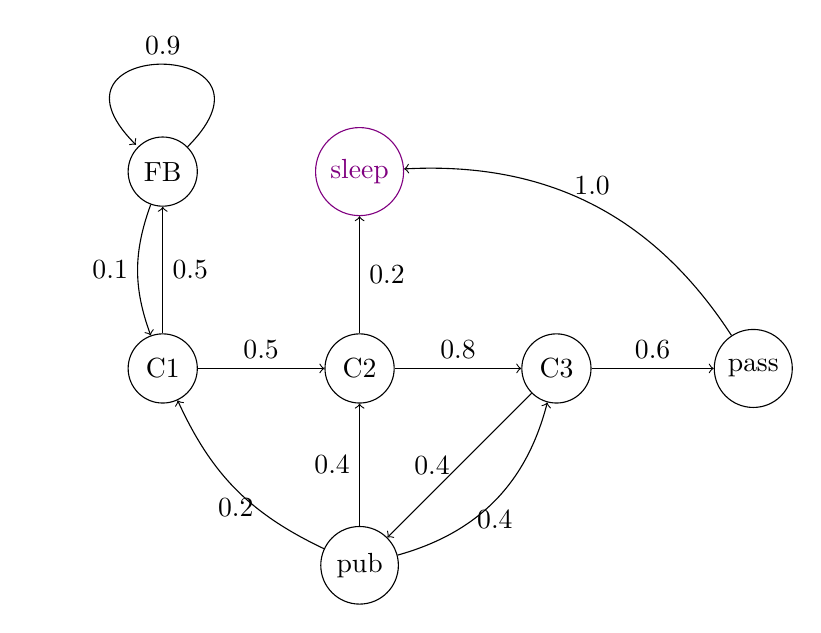
\begin{tikzpicture}[x=2.5cm, y=2.5cm]
                    \node[state] (fb) at (0, 0) {FB};
                    \node[state] (c1) at (0, -1) {C1};
                    \node[state] (c2) at (1, -1) {C2};
                    \node[state] (c3) at (2, -1) {C3};
                    \node[state] (p) at (3, -1) {pass};
                    \node[state] (pub) at (1, -2) {pub};
                    \node[state, violet] (sleep) at (1, 0) {sleep};

                    \draw
                    (c1) edge[->, right] node{$0.5$} (fb)
                    (fb) edge[->, bend right=20, left] node{$0.1$} (c1)
                    (fb) edge[loop, ->, above] node{$0.9$} (fb)
                    (c1) edge[->, above] node{$0.5$} (c2)
                    (c2) edge[->, above] node{$0.8$} (c3)
                    (c3) edge[->, above] node{$0.6$} (p)
                    (p) edge[->, bend right=30, above] node{$1.0$} (sleep)
                    (c2) edge[->, right] node{$0.2$} (sleep)
                    (pub) edge[->, bend left=20, below] node{$0.2$} (c1)
                    (pub) edge[->, left] node{$0.4$} (c2)
                    (pub) edge[->, bend right=30, below] node{$0.4$} (c3)
                    (c3) edge[->, left] node{$0.4$} (pub);
                \end{tikzpicture}
            \end{center}
            The entries must be probabilities (hence between 0 and 1).
            The matrix defines transition probabilities from all states $s$ to all successor states $s^\prime$.
            Since all probabilities have to be accounted for (all rows of the matrix sum to 1) - after leaving $s$, we need to end up somewhere, which could also mean returning to $s$;
            $$\summation{s^\prime}{} \mathcal{P}_{ss^\prime} = 1$$
            In the example above, the probability of going to sleep after C2 (class 2) in the morning could be different depending on the time of day (i.e. constantly changing).
            If $P[s_{t + 1}\ \vline\ s_t]$ doesn't depend on $t$, but rather just the origin and destination states, then the Markov chain is stationary or homogenous.
            \subsubsection*{Markov Reward Process}
                A Markov Reward Process is a Markov chain which emits rewards (the reward hypothesis states that all of what we think of as goals and purposes can be thought of as the maximisation of the expected value of the cumulative sum of a scalar signal known as reward); hence a tuple $(\mathcal{S}, \mathcal{P}, \mathcal{R}, \gamma)$.
                This has the following components;
                \begin{itemize}
                    \itemsep0em
                    \item $\mathcal{S}$ \hfill a set of states
                    \item $\mathcal{P}_{ss^\prime}$ \hfill a state transition probability matrix
                    \item $\mathcal{R}_s = \mathbb{E}[r_{t + 1}\ \vline\ S_t = s]$
                        \subitem an expected immediate reward, collected upon departing state $s$ (collection occurs at time $t + 1$, we are at state $s$ at time $t$)
                    \item $\gamma \in [0, 1]$ \hfill discount factor
                \end{itemize}
                We can define the return $R_t$ as the total discounted reward from time-step $t$ (note that we use $t + 1$ as the first element, since it's collected at $t + 1$);
                $$R_t = r_{t + 1} + \gamma r_{t + 2} + \dots = \summation{k = 0}{\infty} \gamma^k r_{t + k + 1}$$
                The factor $\gamma$ is how we discount the present value of future rewards; the value of receiving a reward $r$ after $k + 1$ time steps is $\gamma^k r$, valuing immediate reward higher than a delayed reward - hence $\gamma$ closer to 0 leads to short-sighted evaluation, whereas $\gamma$ closer to 1 leads to far-sighted evaluation (taking future rewards more strongly).

                \medskip
                We can add a reward to the previous example as follows (in \red{red});
                \begin{center}
                    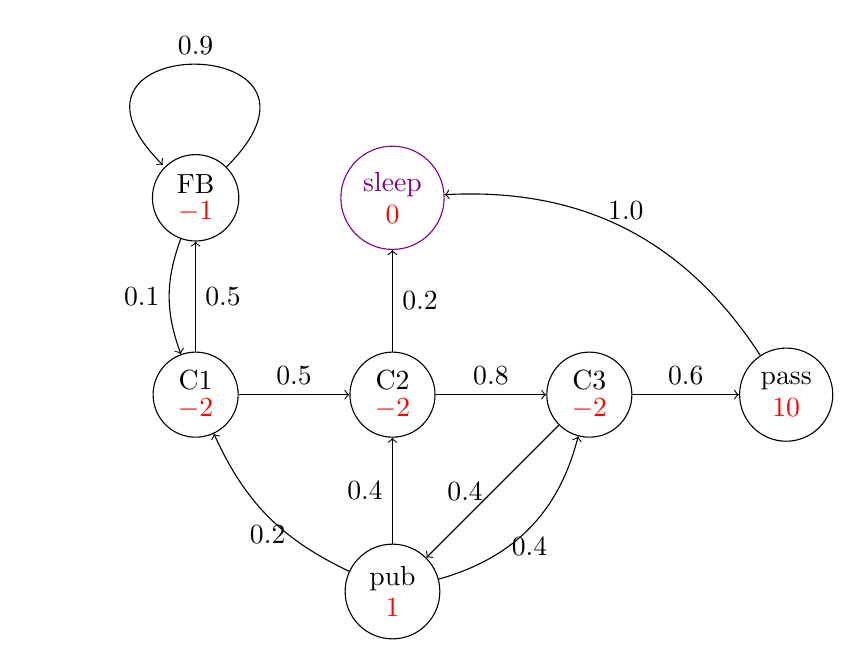
\begin{tikzpicture}[x=2.5cm, y=2.5cm]
                        \node[state] (fb) at (0, 0) {\shortstack{FB\\\red{$-1$}}};
                        \node[state] (c1) at (0, -1) {\shortstack{C1\\\red{$-2$}}};
                        \node[state] (c2) at (1, -1) {\shortstack{C2\\\red{$-2$}}};
                        \node[state] (c3) at (2, -1) {\shortstack{C3\\\red{$-2$}}};
                        \node[state] (p) at (3, -1) {\shortstack{pass\\\red{$10$}}};
                        \node[state] (pub) at (1, -2) {\shortstack{pub\\\red{$1$}}};
                        \node[state, violet] (sleep) at (1, 0) {\shortstack{sleep\\\red{$0$}}};

                        \draw
                        (c1) edge[->, right] node{$0.5$} (fb)
                        (fb) edge[->, bend right=20, left] node{$0.1$} (c1)
                        (fb) edge[loop, ->, above] node{$0.9$} (fb)
                        (c1) edge[->, above] node{$0.5$} (c2)
                        (c2) edge[->, above] node{$0.8$} (c3)
                        (c3) edge[->, above] node{$0.6$} (p)
                        (p) edge[->, bend right=30, above] node{$1.0$} (sleep)
                        (c2) edge[->, right] node{$0.2$} (sleep)
                        (pub) edge[->, bend left=20, below] node{$0.2$} (c1)
                        (pub) edge[->, left] node{$0.4$} (c2)
                        (pub) edge[->, bend right=30, below] node{$0.4$} (c3)
                        (c3) edge[->, left] node{$0.4$} (pub);
                    \end{tikzpicture}
                \end{center}
                For example, consider a certain run, where the starting state $S_1 = \text{C1}$ and $\gamma = \frac{1}{2}$, $T$ is the time to reach the terminal state;
                $$R_1 = r_2 + \gamma r_3 + \dots + \gamma^{T - 2}r_T$$
                Consider the run where the student attends all classes in order and passes; hence C1, C2, C3, pass, sleep;
                $$R_1 = -2 + \frac{1}{2} \cdot -2 + \frac{1}{2}^2 \cdot -2 + \frac{1}{2}^3 \cdot 10$$
                Most MRPs are discounted with $\gamma < 1$, as it's mathematically convenient by avoiding infinite returns in cyclic / infinite processes (by causing convergence).
                It also aids in expressing uncertainty in future rewards.
                A more tangible example is a financial reward, where immediate rewards can be put into a bank and earn interest, similarly, animal decision making shows preference for immediate rewards rather than future rewards.
                \medskip

                We can define the state value function $v(s)$ of a MRP as the expected return $R$ starting from state $s$ at time $t$, thinking of the state as a function parameter;
                $$v(s) = \mathbb{E}[R_t\ \vline\ S_t = s]$$
                The lecture then goes over an example using golf, which is actually quite intuitive.
                \medskip

                The Bellman Equation for MRPs is as follows.
                We can express it in a recurrence relation, as the \violet{immediate reward} and the \teal{discounted return of the successor state}.
                \begin{align*}
                    v(s) & = \mathbb{E}[R_t\ \vline\ S_t = s] \\
                    & = \mathbb{E}[r_{t + 1} + \gamma r_{t + 2} + \gamma^2 r_{t + 3} + \dots\ \vline\ S_t = s] \\
                    & = \mathbb{E}[r_{t + 1} + \gamma(r_{t + 2} + \gamma r_{t + 3} + \dots)\ \vline\ S_t = s] \\
                    & = \mathbb{E}[r_{t + 1} + \gamma R_{t + 1}\ \vline\ S_t = s] \\
                    & = \mathbb{E}[\violet{r_{t + 1}} + \teal{\gamma v(S_{t + 1}})\ \vline\ S_t = s]
                \end{align*}
                The equation can also be written as the sum notation (the previous one was the expectation notation, this has the expectation written out) - there are a total of $n$ of these equations, as there's one for each state;
                $$v(s) = \mathcal{R}_s + \gamma \summation{s^\prime \in S}{} \mathcal{P}_{ss^\prime}v(s^\prime)$$
                As such, this can be written in vector notation as follows, with $\vec{v}$ being $n$-dimensional;
                $$\vec{v} = \mathcal{R} + \gamma \mathcal{P} \vec{v}$$
                This can be directly solved as follows, as it's linear and self-consistent;
                \begin{align*}
                    \vec{v} & = \mathcal{R} + \gamma \mathcal{P} \vec{v} \\
                    (\mathds{1} - \gamma \mathcal{P}) \vec{v} & = \mathcal{R} \\
                    \vec{v} & = (\mathds{1} - \gamma \mathcal{P})^{-1} \mathcal{R}
                \end{align*}
                Since matrix inversion is computationally expensive, being in the order of $n^3$ for $n$ states, a direct solution is only feasibly for small MRPs.
                Iterative methods for solving large MRPs include (and all three will be covered);
                \begin{itemize}
                    \itemsep0em
                    \item dynamic programming
                    \item Monte-Carlo evaluation
                    \item Temporal-Difference learning
                \end{itemize}
            \subsubsection*{Policies}
                A policy $\pi$ is a function of the state, formalising the actions to take at a given state.
                A rigid, deterministic policy can be disadvantageous (e.g. rock, paper, scissors) - exposing the agent to being systematically exploited.
                A policy can be formally described as the conditional probability distribution to execute an action $a \in \mathcal{A}$ given that one is in state $s \in \mathcal{S}$ at time $t$;
                $$\pi_t(a, s) = P[A_t = a\ \vline\ S_t = s]$$
                The general form of the policy is probability, or stochastic, hence $\pi$ is a probability.
                However, if the policy is deterministic (only a single $a$ is possible for state $s$), then $\pi(a, s) = 1$, $\pi(a^\prime, s) = 0,\ \forall a \neq a^\prime$.
                \medskip

                Consider the following example, where there are two actions, $a_1, a_2$ where we either play the lottery (costing 1), or save (not costing anything).
                The two states, $s_1$ and $s_2$ correspond to winning or losing the lottery.
                $$a^* = \argmax_{a_i} \summation{j = 1}{2} \mathcal{R}_{s_j}^{a_j}P[s_j\ |\ a_i]$$
        \subsection*{Markov Decision Process}
            The emphasis decision process, with decision being the key, combines the policies with MRPs.
            The MDP consists of the following;
            \begin{itemize}
                \itemsep0em
                \item $\mathcal{S}$ \hfill state space
                \item $\mathcal{A}$ \hfill action space
                \item $\mathcal{P}_{ss^\prime}^a$ \hfill transition probability $p(s_{t + 1}\ \vline\ s_t, a_t)$
                    \subitem probability of transitioning to the next state $s_{t + 1}$, given the current state $s_t$ and action $a_t$ taken
                \item $\gamma \in [0, 1]$ \hfill discount factor
                \item $\mathcal{R}_{ss^\prime}^a = r(s, a, s^\prime)$ \hfill immediate reward function
                    \subitem in temporal notation, $r_{t + 1} = r(s_{t + 1}, s_t, a_t)$ - reward is collected upon the transition from $s_t$ to $s_{t + 1}$, which occurs at time $t + 1$
                \item $\pi$ \hfill policy, can be either stochastic or deterministic
                    \subitem stochastic is written as the following; $\vec{a} \sim p_\pi(\vec{a}\ \vline\ \vec{s}) = \pi(\vec{a}\ \vline\ \vec{s}) \equiv \pi(a, s)$ - being a probability distribution
                    \subitem deterministic is written as $\vec{a} = \pi(\vec{s})$ (indicator function)
            \end{itemize}
            Note that the transition probability and policy both take the action into account, as parameters.
            We can graphically represent this as follows, with nodes denoting variables, and edges denoting conditional dependencies between these variables;
            \begin{center}
                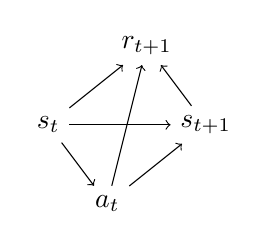
\begin{tikzpicture}]
                    \node (rt1) at (0.25, 0) {$r_{t + 1}$};
                    \node (st) at (-1, -1) {$s_t$};
                    \node (st1) at (1, -1) {$s_{t + 1}$};
                    \node (at) at (-0.25, -2) {$a_t$};

                    \draw
                    (st) edge[->] (at)
                    (st) edge[->] (rt1)
                    (st) edge[->] (st1)
                    (at) edge[->] (rt1)
                    (at) edge[->] (st1)
                    (st1) edge[->] (rt1);
                \end{tikzpicture}
            \end{center}
            This tells us that the action $a_t$ depends on the current state $s_t$, the next state $s_{t + 1}$ depends on both the action and the current state, and the reward $r_{t + 1}$ depends on all three.
            \subsubsection*{Value Function}
                The goodness of a given state is defined with the value function (where $R_t$ is a discounted total return, and $r_{t + k + 1}$ are immediate rewards);
                $$V^\pi(s) = \mathbb{E}_\pi[R_t\ |\ S_t = s] = E\left[\summation{k = 0}{\infty}  \gamma^kr_{t + k + 1}\ \vline\ S_t = s\right]$$
                This is quite similar to the derivation of the Bellman equation for MRPs, but now including the action (see the policies $\pi$).
                Note that expectation is a linear operator, hence we can justify the final line, also note in the penultimate line we separate out the \violet{next reward} from the discounted rewards;
                \begin{align*}
                    V^\pi(s) & = \mathbb{E}_\pi[R_t\ |\ S_t = s] \\
                    & = \mathbb{E}_\pi\left[\summation{k = 0}{\infty} \gamma^kr_{t + k + 1}\ \vline\ S_t = s\right] \\
                    & = \mathbb{E}_\pi\left[\violet{r_{t + 1}} + \gamma\summation{k = 0}{\infty} \gamma^kr_{t + k + 2}\ \vline\ S_t = s\right] \\
                    & = \mathbb{E}[r_{t + 1}\ |\ S_t = s] + \gamma\mathbb{E}\left[\summation{k = 0}{\infty} \gamma^kr_{t + k + 2}\ \vline\ S_t = s\right]
                \end{align*}
            \subsubsection*{Backup Diagrams}
                We start at a white node, at a particular state $s$ (since we are conditioning on a particular state $S_t = s$).
                From this state, we can take several actions, represented by the black nodes, which leads us to following states $s^\prime$, with a reward $r$.
                This state value information is transferred back up to $s$ from its successor state $s^\prime$, performing the \textbf{update} or \textbf{backup} operation at the heart of the reinforcement learning method.
                \begin{center}
                    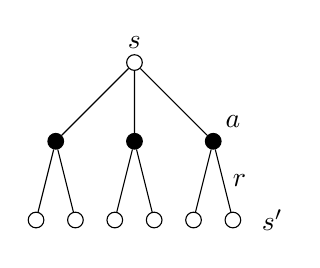
\begin{tikzpicture}
                        \node[budw] (o) at (0, 0) {};
                        \node[budb] (ol) at (-1, -1) {};
                        \node[budb] (oc) at (0, -1) {};
                        \node[budb] (or) at (1, -1) {};
                        \node[budw] (oll) at (-1.25, -2) {};
                        \node[budw] (olr) at (-0.75, -2) {};
                        \node[budw] (ocl) at (-0.25, -2) {};
                        \node[budw] (ocr) at (0.25, -2) {};
                        \node[budw] (orl) at (0.75, -2) {};
                        \node[budw] (orr) at (1.25, -2) {};

                        \draw
                        (o) -- (ol)
                        (o) -- (oc)
                        (o) -- (or)
                        (ol) -- (oll)
                        (ol) -- (olr)
                        (oc) -- (ocl)
                        (oc) -- (ocr)
                        (or) -- (orl)
                        (or) edge[right] node{$r$} (orr);

                        \node at (0, 0.25) {$s$};
                        \node at (1.25, -0.75) {$a$};
                        \node at (1.75, -2) {$s^\prime$};
                    \end{tikzpicture}
                \end{center}
                In order to calculate the value of state $s$, we need to average over all possible traces, which is what's going on behind the scenes in the expectation operator - an average weighted by probabilities.
                All of which live inside the MDP;
                \begin{itemize}
                    \itemsep0em
                    \item probability of the chosen action $a$ is given by the policy $P[a\ \vline\ s] = \pi(a, s)$
                    \item probability of a transition to $s^\prime$ is given by the transition probability $P[s^\prime\ \vline\ s, a] = \mathcal{P}_{ss^\prime}^a$
                    \item instantaneous reward $r$ is given by the reward function $r(s, a, s^\prime) = \mathcal{R}_{ss^\prime}^a$
                    \item the value of the next state $s^\prime$, weighted by the probability functions is given recursively by $v(s^\prime)$
                \end{itemize}
                Writing it out, note that we have the value function of the state $s^\prime$ in \violet{violet};
                \begin{align*}
                    \mathbb{E}[r_{t + 1}\ |\ S_t = s] & = \summation{a \in \mathcal{A}}{} P\left[a\ |\ s\right] \left(\summation{s^\prime \in \mathcal{S}}{} P[s^\prime\ |\ s, a] r(s, a, s^\prime)\right) \\
                    \mathbb{E}\left[\summation{k = 0}{\infty} \gamma^kr_{t + k + 2}\ \vline\ S_t = s\right] & = \summation{a \in \mathcal{A}}{} P\left[a\ |\ s\right] \left(\summation{s^\prime \in \mathcal{S}}{} P[s^\prime\ |\ s, a] \violet{\summation{k = 0}{\infty} \gamma^kr_{t + k + 2}}\right) \\
                    V^\pi(s^\prime) & = \mathbb{E}[R_{t + 1}\ \vline\ S_{t + 1} = s^\prime] \\
                    & = \mathbb{E}\left[\summation{k = 0}{\infty} \gamma^kr_{t + k + 2}\ \vline\ S_{t + 1} = s^\prime\right]
                \end{align*}
                We can combine all of this as follows;
                \begin{align}
                    V^\pi(s) & = \mathbb{E}_\pi [R_t\ |\ S_t = s] \\
                    & = \mathbb{E}_\pi\left[\summation{k = 0}{\infty} \gamma^kr_{t + k + 1}\ \vline\ S_t = s\right] \\
                    & = \mathbb{E}_\pi\left[r_{t + 1} + \gamma\summation{k = 0}{\infty} \gamma^kr_{t + k + 2}\ \vline\ S_t = s\right] \\
                    & = \summation{a \in \mathcal{A}}{} \pi(a, s) \left(\summation{s^\prime \in \mathcal{S}}{} \mathcal{P}_{ss^\prime}^a \left(\mathcal{R}_{ss^\prime}^a + \gamma\mathbb{E}_\pi\left[\summation{k = 0}{\infty} \gamma^kr_{t + k + 2}\ \vline\ S_{t + 1} = s^\prime\right]\right)\right) \\
                    & = \summation{a \in \mathcal{A}}{} \pi(a, s) \summation{s^\prime \in \mathcal{S}}{} \mathcal{P}_{ss^\prime}^a (\mathcal{R}_{ss^\prime}^a + \gamma V^\pi(s^\prime))
                \end{align}
                Here we are performing the following steps;
                \begin{enumerate}[(1)]
                    \itemsep0em
                    \setcounter{enumi}{1}
                    \item write the definition of the return
                    \item separate immediate reward
                    \item split expectation in two, as it's a linear operator, also write out expectation weighted by probabilities, and using proper notation for policies $\pi(a, s)$, transition probabilities $\mathcal{P}_{ss^\prime}^a$, and reward function $\mathcal{R}_{ss^\prime}^a$
                    \item substitute with recursive definition
                \end{enumerate}
                This is a consistency condition imposed on the value function and also has a unique solution.
                Computing the value function for an arbitrary policy is known as policy evaluation or prediction problem.
                Now, we need to iterate applications to obtain better estimates - note that the subscripts in $V_1(s), V_2(s), \dots, V_k(s)$ denote iterations, not states; this is guaranteed to converge.
                This is known as iterative policy evaluation.
                A stopping condition can be achieved by checking that the \textbf{largest} change in the value function, between iterations, is below a certain small threshold.
                This can be formalised as follows - note that the value function is on a particular policy;
                \begin{enumerate}
                    \itemsep0em
                    \item input $\pi$, the policy to be evaluated
                    \item initialise $V(s) = 0$ for all $s \in \mathcal{S}^+$
                    \item repeat the following until $\Delta < \theta$ (where $\theta$ is some small positive number)
                        \begin{enumerate}
                            \itemsep0em
                            \item $\Delta \leftarrow 0$
                            \item for each $s \in \mathcal{S}$;
                                \begin{enumerate}
                                    \itemsep0em
                                    \item $v \leftarrow V(s)$ \hfill store old value
                                    \item $V(s) \leftarrow \summation{a \in \mathcal{A}}{} \pi(a, s) \summation{s^\prime \in \mathcal{S}}{} \mathcal{P}_{ss^\prime}^a (\mathcal{R}_{ss^\prime}^a + \gamma V^\pi(s^\prime))$ \hfill sweep through successors, a full backup
                                    \item $\Delta \leftarrow \max(\Delta, | v - V(s) |)$
                                \end{enumerate}
                        \end{enumerate}
                    \item output $V \approx V^\pi$
                \end{enumerate}
                Note that this replaces values, in place, converging faster than a two-array method, which would have both an old and new array.
            \subsubsection*{Stair Climbing MDP}
                Consider the following example; for brevity, a \violet{violet} edge means a Right action, and a \teal{teal} edge denotes a Left action.
                $P$ and $G$ are both absorbing / terminal states, assume we start at $s_3$ with $\gamma = 0.9$, an unbiased policy (such that all actions are equally probable) with $\pi(s, L) = \pi(s, R) = 0.5$, hence randomly selecting actions.
                \begin{center}
                    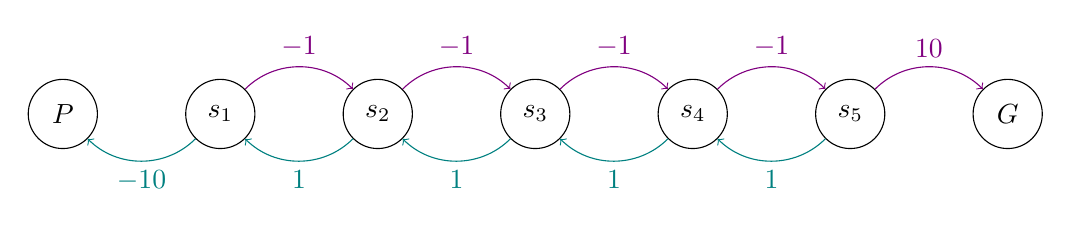
\begin{tikzpicture}[x=2cm]
                        \node[state] (p) at (0, 0) {$P$};
                        \node[state] (s1) at (1, 0) {$s_1$};
                        \node[state] (s2) at (2, 0) {$s_2$};
                        \node[state] (s3) at (3, 0) {$s_3$};
                        \node[state] (s4) at (4, 0) {$s_4$};
                        \node[state] (s5) at (5, 0) {$s_5$};
                        \node[state] (g) at (6, 0) {$G$};
                        \draw
                        (s1) edge[->, violet, above, bend left=45] node{$-1$} (s2)
                        (s2) edge[->, violet, above, bend left=45] node{$-1$} (s3)
                        (s3) edge[->, violet, above, bend left=45] node{$-1$} (s4)
                        (s4) edge[->, violet, above, bend left=45] node{$-1$} (s5)
                        (s5) edge[->, violet, above, bend left=45] node{$10$} (g)
                        (s5) edge[->, teal, below, bend left=45] node{$1$} (s4)
                        (s4) edge[->, teal, below, bend left=45] node{$1$} (s3)
                        (s3) edge[->, teal, below, bend left=45] node{$1$} (s2)
                        (s2) edge[->, teal, below, bend left=45] node{$1$} (s1)
                        (s1) edge[->, teal, below, bend left=45] node{$-10$} (p);
                    \end{tikzpicture}
                \end{center}
                Note that in the first iteration, the only changes are to $s_1$ and $s_5$, as they are the only ones with successor states that have different rewards (all other states will cancel out), also note the symmetry stemming from the symmetrical problem.
                \begin{center}
                    \begin{tabular}{|c|ccccccc|}
                        $V$ & $P$ & $s_1$ & $s_2$ & $s_3$ & $s_41$ & $s_5$ & $G$ \\
                        \hline
                        $V_0$ & $0$ & $0$ & $0$ & $0$ & $0$ & $0$ & $0$ \\
                        $V_1$ & $0$ & $-5.5$ & $0$ & $0$ & $0$ & $5.5$ & $0$ \\
                        $V_2$ & $0$ & $-5.5$ & $-2.48$ & $0$ & $2.48$ & $5.5$ & $0$ \\
                        $V_2$ & $0$ & $-6.61$ & $-2.48$ & $0$ & $2.48$ & $6.61$ & $0$ \\
                        $\vdots$ & & & & & & & \\
                        $V_\infty$ & $0$ & $-6.9$ & $-3.1$ & $0$ & $3.1$ & $6.9$ & $0$
                    \end{tabular}
                \end{center}
                Note that we are still equally likely to go to the left, despite being significantly worse; thus knowing the value of the policy can improve the policy.
            \subsubsection*{State-Action Value Function}
                This takes in two parameters; a state $s$ and an action $a$, giving us a function that determines the value of taking a certain action at a state.
                $$Q^\pi(s, a) = \mathbb{E}[R_t\ |\ S_t = s, A_t = a] = \mathbb{E}\left[\summation{k = 0}{\infty} \gamma^k r_{t + k + 1}\ \vline\ S_t = s, A_t = a\right]$$
                The relation between the state value function and this is;
                $$V^\pi(s) = \summation{a \in \mathcal{A}}{} \pi(s, a)Q^\pi(s, a)$$
            \subsubsection*{Bellman Optimality Equations}
                Previously, we discussed arbitrary policies.
                However, we can define an ordering on policies (such that some policies are better than others) by saying a policy is better than, or equal to, another policy if its expected return is also greater than or equal to the other policy for all states; $\pi \geq \pi^\prime$ iff $\forall s \in \mathcal{S}\ [V^\pi(s) \geq V^{\pi^\prime}(s)]$.
                As such, the optimal value function is defined as;
                $$V^*(s) = \max_\pi V^\pi(s), \forall s \in \mathcal{S}$$
                We call the policy $\pi^*$ which maximises the value function the optimal policy; there will always be at least one, but multiple can exist.
                Similarly, there is also an optimal state-action value function;
                $$Q^*(s, a) = \max_\pi Q^\pi(s, a), \forall s \in \mathcal{S}, a \in \mathcal{A} = \mathbb{E}[r_{t + 1} + \gamma V^*(s_{t + 1})\ |\ S_t = s, A_t = a]$$
                The Bellman equations for these are called Bellman Optimality equations.
                \medskip

                We have already seen the backup diagram for the value function, and the state-action value function backup diagram is similar (you can think of them as the black nodes and its children);
                \begin{center}
                    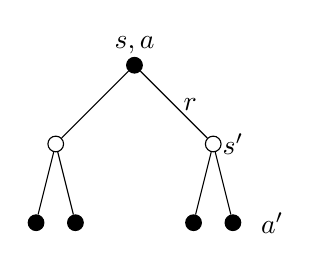
\begin{tikzpicture}
                        \node[budb] (o) at (0, 0) {};
                        \node[budw] (ol) at (-1, -1) {};
                        \node[budw] (or) at (1, -1) {};
                        \node[budb] (oll) at (-1.25, -2) {};
                        \node[budb] (olr) at (-0.75, -2) {};
                        \node[budb] (orl) at (0.75, -2) {};
                        \node[budb] (orr) at (1.25, -2) {};

                        \node at (0, 0.25) {$s, a$};
                        \node at (1.25, -1) {$s^\prime$};
                        \node at (1.75, -2) {$a^\prime$};

                        \draw
                        (o) -- (ol)
                        (o) edge[right] node{$r$} (or)
                        (ol) -- (oll)
                        (ol) -- (olr)
                        (or) -- (orl)
                        (or) -- (orr);
                    \end{tikzpicture}
                \end{center}
                The white nodes are associated with the value function $V^\pi(s)$, the black nodes with the value-action function $Q^\pi(s, a)$, and the paths between the nodes taken with probability $\pi(s, a)$.
                The relationship for the function, on just the value function backup diagram can be shown as follows;
                \begin{center}
                    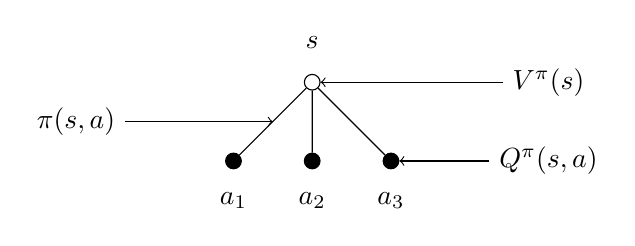
\begin{tikzpicture}
                        \node[budw] (o) at (0, 0) {};
                        \node[budb] (ol) at (-1, -1) {};
                        \node[budb] (oc) at (0, -1) {};
                        \node[budb] (or) at (1, -1) {};

                        \node at (0, 0.5) {$s$};
                        \node at (-1, -1.5) {$a_1$};
                        \node at (0, -1.5) {$a_2$};
                        \node at (1, -1.5) {$a_3$};

                        \node (v) at (3, 0) {$V^\pi(s)$};
                        \node (q) at (3, -1) {$Q^\pi(s, a)$};
                        \node (p) at (-3, -0.5) {$\pi(s, a)$};

                        \draw
                        (o) -- (ol)
                        (o) -- (oc)
                        (o) -- (or)
                        (v) edge[->] (o)
                        (q) edge[->] (or)
                        (p) edge[->] (-0.5, -0.5);
                    \end{tikzpicture}
                \end{center}
                If we want the optimal value for a state, only actions that give the highest value should be chosen;
                \setcounter{equation}{0}
                \begin{align}
                    V^*(s) & = \max_{a \in \mathcal{A}} \summation{a \in \mathcal{A}}{} \pi(s, a) Q^\pi(s, a) \\
                    & = \max_a Q^{\pi^*}(s, a) \\
                    & = \max_a \mathbb{E}[R_t\ |\ S_t = s, A_t = a] \\
                    & = \max_a \mathbb{E}\left[\summation{k = 0}{\infty} \gamma^k r_{t + k + 1}\ \vline\ S_t = s, A_t = a\right] \\
                    & = \max_a \mathbb{E}\left[r_{t + 1} + \gamma\summation{k = 0}{\infty} \gamma^k r_{t + k + 2}\ \vline\ S_t = s, A_t = a\right] \\
                    & = \max_a \mathbb{E}[r_{t + 1} + \gamma V^*(s_{t + 1})\ |\ S_t = s, A_t = a] \\
                    & = \max_a \summation{s^\prime}{} P[s^\prime\ |\ s, a] (r(s, a, s^\prime) + \gamma V^*(s^\prime)) \\
                    & = \max_a \summation{s^\prime}{} \mathcal{P}_{ss^\prime}^a (\mathcal{R}_{ss^\prime}^a + \gamma V^*(s^\prime))
                \end{align}
                We perform the following steps;
                \begin{enumerate}[(1)]
                    \itemsep0em
                    \setcounter{enumi}{2}
                    \item write down definition of state-action value function, being the expected return conditioned on $s$ and $a$
                    \item perform usual expansion with the maximum on the left
                    \setcounter{enumi}{6}
                    \item replace with probabilities
                \end{enumerate}
                There is no reference to any particular policy and must therefore be satisfied by all optimal policies.
                The optimality equation expresses that the value of a state under an optimal policy is equal to the expected return of the best action from the state.
                This can be done similarly for $Q^*$, except the maximum is now on the inside;
                \begin{align*}
                    Q^*(s, a) & = \mathbb{E}\left[r_{t + 1} + \gamma\max_{a^\prime} Q^*(s_{t + 1}, a^\prime)\ \vline\ S_t = s, A_t = a\right] \\
                    & = \summation{s^\prime}{} \mathcal{P}_{ss^\prime}^a \left(\mathcal{R}_{ss^\prime}^a + \gamma\max_{a^\prime} Q^*(s^\prime, a^\prime)\right)
                \end{align*}
                Notice that the equation doesn't require $\pi^*$ at all, which is useful as we don't need to know the optimal policy to solve the optimality equations.
                For finite MDPs, this equation has a unique solution, independent of the policy.
                The bellman optimality equation is a set of $N$ non-linear equations, where $N = |\mathcal{S}|$, with $N$ unknowns.
                \medskip

                An explicit solution for the optimality equation provides one route for an optimal policy - however we are often going to encounter a high-dimensional problem (large state space).
                This also assumes the following, which are rarely true;
                \begin{itemize}
                    \itemsep0em
                    \item we accurately know the dynamics of the environment
                    \item we have the resources to find the solution
                    \item the Markov property
                \end{itemize}
                We therefore often settle for approximate solutions.
                \medskip

                The BOE convergence theorem states that for an MDP with finite state and action space, the optimality equations have a unique solution and the values produced by iteration converge to the solution of the equations.
                The proof of this rests on the Banach Fixed Point / Contraction Mapping Theorem.
        \subsection*{October 14 - Live Lecture}
            AI is a question; how do we build systems that solve tasks for which humans need intelligence?
            On the other hand, machine learning is the answer to the AI question, including methods, algorithms and data structures that learn to solve these tasks from data.
            Big data means methods, processing, and assessing very large data, broken into data science (how to ask interesting questions about the data using methods from ML) and data engineering (how to build Hadoop systems, fitting data in memory, etc.).
            \medskip

            Reinforcement penalises negative behaviour and rewards behaviour that actually works; a goal structure is given.
            RL solves control problems; choosing the optimal action at the right time.
            \medskip

            The general framework for reinforcement learning contains the following;
            \begin{itemize}
                \itemsep0em
                \item agent interacts with the environment to gain knowledge; action is fundamental
                \item explore and receive rewards; exploration involves trying actions (can also be nothing), receiving rewards, penalty, both long-term and short-term
                \item actions have an effect on the state of the environment
                \item choose actions to maximise long-term rewards
            \end{itemize}
            Control is sequential decision making, and optimal control which minimises a cost, or maximises a reward.
            RL involves learning an optimal control of an unknown system.
            \medskip

            The session then goes into a refresher on probabilities.
\end{document}